% Document class and basic setup
\documentclass[10pt]{exam}
% \usepackage[utf8]{inputenc}
% \usepackage[T1]{fontenc}

% Page layout and geometry
\usepackage[margin=0.25in, includefoot, includehead]{geometry}
\usepackage{microtype}

% Font packages - XeLaTeX/LuaLaTeX vs pdfLaTeX compatibility
\usepackage{ifxetex,ifluatex}
\ifxetex
\usepackage{fontspec}
\setmainfont{Linux Libertine O}[
  Ligatures=TeX,
  Numbers=OldStyle
]
\setsansfont{Linux Biolinum O}[
  Ligatures=TeX,
  Numbers=OldStyle
]
% \setmonofont{Latin Modern Mono}[Scale=MatchLowercase]
\setmonofont{DejaVu Sans Mono}[Scale=MatchLowercase]
\else\ifluatex
\usepackage{fontspec}
\setmainfont{Linux Libertine O}[
  Ligatures=TeX,
  Numbers=OldStyle
]
\setsansfont{Linux Biolinum O}[
  Ligatures=TeX,
  Numbers=OldStyle
]
\setmonofont{Latin Modern Mono}[Scale=MatchLowercase]
\else
\usepackage{libertine}
\fi\fi

% Math packages
\usepackage{amsmath,amssymb,amsthm}
\usepackage{mathtools}
\usepackage{bm}
\usepackage{accents}

% List and enumeration
\usepackage[shortlabels]{enumitem}
\usepackage{multicol}

% Graphics and figures
\usepackage{graphicx}
\usepackage{tikz}
\usepackage{pgfplots}
\pgfplotsset{compat=1.18}
\usetikzlibrary{shapes}
\usepackage{pgfplots}
\pgfplotsset{compat=1.18}
% \usepackage{svg}
\usepackage{graphicx}
\usepackage{float}
\usepackage{wrapfig}

% Tables and arrays
\usepackage{booktabs}
\usepackage{multirow}
\usepackage{nicematrix}

% Color and highlighting
\usepackage{xcolor}
\definecolor{answerboxcolor}{RGB}{255,245,245} % Very light red background
\usepackage{empheq}

% Captions and references
\usepackage[hypcap=false,font=small,labelfont=bf,tableposition=top]{caption}
\usepackage{subcaption}
\usepackage[colorlinks=true, linkcolor=blue, urlcolor=blue]{hyperref}
\usepackage{cleveref}

% Units and chemistry
\usepackage{siunitx}
\sisetup{
  group-digits=integer,
  group-minimum-digits=3,
  group-separator={,}
}
\DeclareSIUnit\angstrom{\text{\AA}} % \angstrom is depracted, so define it here.
\usepackage[version=4]{mhchem}
\usepackage{chemformula}

% Code listings
\usepackage{minted}
\usepackage{listings}
\AtBeginEnvironment{minted}{
\fontsize{8}{10}\selectfont}

% Utility packages
\usepackage{cancel}
\usepackage{etoolbox}
\usepackage{pdfpages}
\usepackage{blindtext}
\usepackage{lipsum}

% Header and footer setup using exam class commands
% The exam class provides its own header/footer system
\lhead{\textbf{MSEN 640-600}}
\chead{\textbf{Homework \#1}}
\rhead{\textbf{Nathaniel Thomas}}
\lfoot{}
\cfoot{\thepage}
\rfoot{}

% Add header rule
\headrule

% Custom commands
\newcommand{\fahrenheit}{^\circ{F}}
\newcommand*\widefbox[1]{\fbox{\hspace{2em}#1\hspace{2em}}}
\newcommand{\msout}[1]{\text{\sout{$#1$}}}

% SI Units
\DeclareSIUnit\year{y}

% Professional boxed answer environment
% Creates uniform, centered answer boxes with light red background
\newcommand{\boxedanswer}[1]{
  \begin{center}
    \fcolorbox{black}{answerboxcolor}{%
      \begin{minipage}{0.85\textwidth}
        \vspace{0.5em}
        #1
        \vspace{0.5em}
      \end{minipage}%
    }
  \end{center}
  \vspace{0.5em}
}

% Alternative boxed answer for nested environments (like enumerate)
\newcommand{\boxedanswersmall}[1]{
  \begin{center}
    \fcolorbox{black}{answerboxcolor}{%
      \begin{minipage}{0.75\textwidth}
        \vspace{0.3em}
        #1
        \vspace{0.3em}
      \end{minipage}%
    }
  \end{center}
  \vspace{0.3em}
}

% Additional SI unit for Fahrenheit
\DeclareSIUnit\fahrenheit{\degree F}

\begin{document}

% Include title page
% Title page with no headers/footers
\thispagestyle{empty}

\begin{titlepage}
  \begin{center}
    \vspace*{2cm}

    % Main title
    \Huge
    \textbf{Homework \#1}

    \vspace{0.8cm}

    % Course information
    \LARGE
    MSEN 640-600

    \vspace{2cm}

    % Author information
    \Large
    \textbf{Prepared by:}\\[0.5cm]
    \huge
    \textbf{Nathaniel Thomas}

    \vspace{1cm}

    \Large
    \textbf{Prepared for:}\\[0.5cm]
    \large
    Dr. Xiaofeng Qian

    \vfill

    % University logo
    
\includegraphics[width=0.4\textwidth]{"./assets/a&m_logo.pdf"}

    \vspace{1cm}

    % University and date information
    \Large
    Materials Science \& Engineering\\
    Texas A\&M University\\
    \vspace{0.5cm}
    \large
    September 12, 2025

  \end{center}
\end{titlepage}


\pagebreak

\section*{Problem 2.4.1}

Which of the following differential equations is linear, in the sense
that, if some function $\psi(z)$ is a
solution (and this may well be a different function for each equation
below), so also is the function
$\psi(z) = a\psi(z)$, where $a$ is an arbitrary constant? Justify your answers.

\begin{enumerate}[(i)]
  \item $z\frac{d\psi(z)}{dz} + g(z)\psi(z) = 0$ where $g(z)$ is some
    specific function

    \boxedanswersmall{

      This equation is linear, as the term $\psi(z)$ does not appear in any
      order higher than first order. As a result, $\psi(z)$ and $a\psi(z)$ are
      both valid solutions, given that $a$ is some constant.
    }

  \item $\psi(z)\frac{d\psi(z)}{dz} + \psi(z) = 0$

    \boxedanswersmall{
      This equation is not linear. The term $\psi(z)\frac{d\psi(z)}{dz}$ is not
      first order in $\psi$. As a result, $\psi(z)$ and $a\psi(z)$ may not both
      be valid solutions, given that $a$ is some constant.
    }

\end{enumerate}

\pagebreak

\section*{Problem 2.6.1}

An electron is in a potential well of thickness \SI{1}{\nano\meter},
with infinitely high potential barriers on either
side. It is in the lowest possible energy state in this well. What
would be the probability of finding the
electron between \SI{0.1}{\nano\meter} and \SI{0.2}{\nano\meter} from
one side of the well?

\boxedanswer{
  \centering
  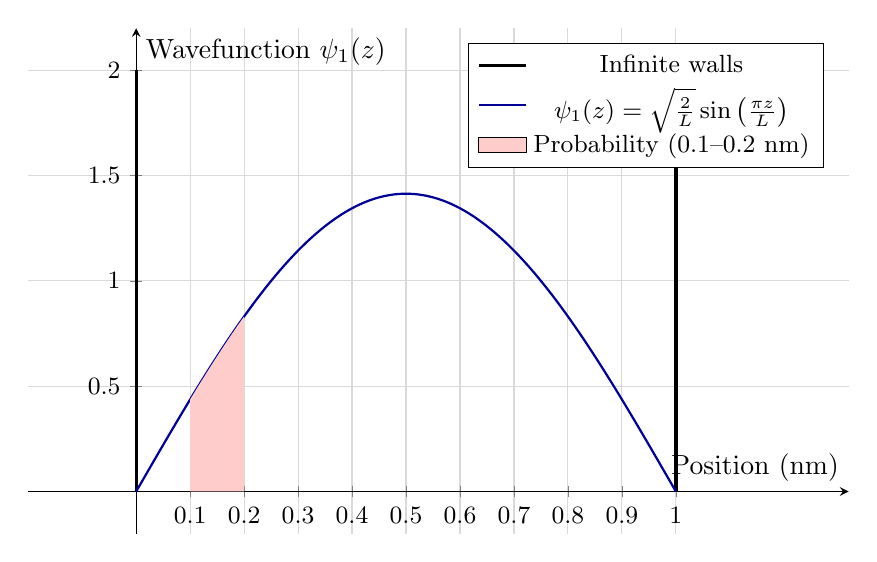
\begin{tikzpicture}
  \begin{axis}[
      xlabel={Position (nm)},
      ylabel={Wavefunction $\psi_1(z)$},
      xmin=-0.2, xmax=1.32,
      ymin=-0.2, ymax=2.2,
      grid=major,
      grid style={gray!30},
      axis lines=middle,
      width=12cm,
      height=8cm,
      xtick={0, 0.1, 0.2, 0.3, 0.4, 0.5, 0.6, 0.7, 0.8, 0.9, 1.0},
      xticklabel style={font=\small},
      yticklabel style={font=\small},
      legend pos=north east,
      legend style={font=\small}
    ]
    % Infinite potential walls (vertical lines)
    \addplot[black, very thick, domain=-0.2:2, samples=2] {-1}; %
    % \addlegendimage{black, very thick}
    \addlegendentry{Infinite walls}
    \draw[black, very thick] (axis cs:0,0) -- (axis cs:0,2);
    \draw[black, very thick] (axis cs:1,0) -- (axis cs:1,2);

    % Ground state wavefunction psi_1(z) = A_1 * sin(pi*z/L)
    % For L = 1 nm, A_1 = sqrt(2/L) = sqrt(2) for normalization
    \addplot[
      domain=0:1,
      samples=200,
      thick,
      blue!60!black
    ] {sqrt(2)*sin(deg(pi*x))};

    % Shaded area under the curve between 0.1 and 0.2 nm
    \addplot[
      domain=0.1:0.2,
      samples=100,
      fill=red!20,
      draw=none,
      area legend
    ] {sqrt(2)*sin(deg(pi*x))} \closedcycle;

    % Add legend entries
    \addlegendentry{$\psi_1(z) =
    \sqrt{\frac{2}{L}}\sin\left(\frac{\pi z}{L}\right)$}
    \addlegendentry{Probability (0.1--0.2 nm)}

    % Add wall labels
    \node[black, above] at (axis cs:1,1.8) {\small Wall};
  \end{axis}
\end{tikzpicture}

  \vspace{0.5em}
  \captionof{figure}{Graph of the ground-state wavefunction for an electron
  positioned within an infinite-potential \SI{1}{\nano\meter} well.}

  \begin{align*}
    p &= \int_{z_1}^{z_2} |\psi_1(z)|^2dz \\
    &
    \begin{aligned}
      \psi_n(z) &= \frac{2}{L_z}\sin\left(\frac{n\pi z}{L_z}\right)
      \\
      &
      \begin{aligned}
        L_z &= \SI{1}{\nano\meter} \\
        n &= 1 \\
      \end{aligned} \\
      \psi_n(z) &=
      \frac{2}{(\SI{1}{\nano\meter})}\sin\left(\frac{(1)\pi
      z}{(\SI{1}{\nano\meter})}\right) \\
      \psi_n(z) &= 2\sin\left(\pi z\right) \\
    \end{aligned} \\
    p &= \int_{z_1}^{z_2} 2\sin^2\left(\pi z\right)dz \\
    p &= \int_{z_1}^{z_2} 2[1 - \cos^2\left(\pi z\right)]dz \\
    &
    \begin{aligned}
      \cos^2\left(\pi z\right) &= \frac{\cos2\theta}{2} + \frac{1}{2} \\
      z_1 &= \SI{0.1}{\nano\meter} \\
      z_2 &= \SI{0.2}{\nano\meter} \\
    \end{aligned} \\
    p &= \int_{z_1}^{z_2} [1 - \cos\left(2\pi z\right)]dz \\
    p &= \left[z - \frac{\sin(2\pi
    z)}{2\pi}\right]_{\SI{1}{\nano\meter}}^{\SI{0.2}{\nano\meter}} \\
    p &= \left[\left(\SI{0.2}{\nano\meter} -
      \frac{\sin(2\pi(\SI{0.2}{\nano\meter}))}{2\pi}\right) -
      \left(\SI{0.1}{\nano\meter} -
    \frac{\sin(2\pi(\SI{0.1}{\nano\meter}))}{2\pi}\right)\right] \\
    \Aboxed{p &= 0.042184}
  \end{align*}
}

\pagebreak

\section*{Problem 2.6.2}

Which of the following functions have a definite parity relative to
the point $x = 0$ (i.e., we are
interested in their symmetry relative to $x = 0$)? For those that
have a definite parity, state whether it
is even or odd.

\begin{enumerate}[(i)]
  \item $\sin(x)$

    \boxedanswersmall{
      \centering
      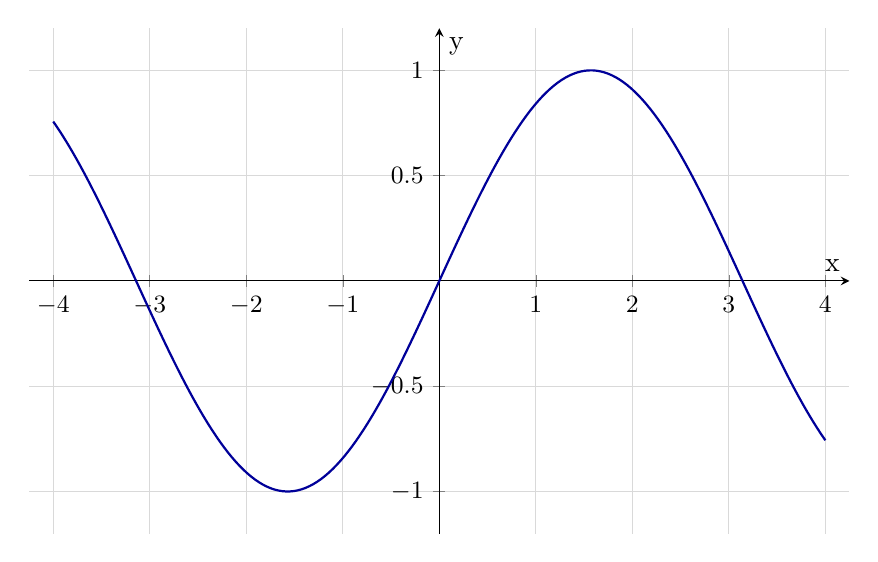
\begin{tikzpicture}
  \begin{axis}[
      xlabel={x},
      ylabel={y},
      xmin=-4.25, xmax=4.25,
      ymin=-1.2, ymax=1.2,
      grid=major,
      grid style={gray!30},
      axis lines=middle,
      width=12cm,
      height=8cm,
      xticklabel style={font=\small},
      yticklabel style={font=\small},
      legend pos=north east,
      legend style={font=\small}
    ]

    \addplot[
      domain=-4:4,
      samples=200,
      thick,
      blue!60!black
    ] {sin(deg(x))};

  \end{axis}
\end{tikzpicture}

      \vspace{0.5em}
      \captionof{figure}{Graph of $y = \sin(x)$.}

      $\sin(x)$ has a definite parity around $x = 0$. $\sin(x) =
      -\sin(-x)$, meaning that $\sin(x)$ is an odd function.

    }

  \item $\exp(ix)$

    \boxedanswersmall{
      \centering
      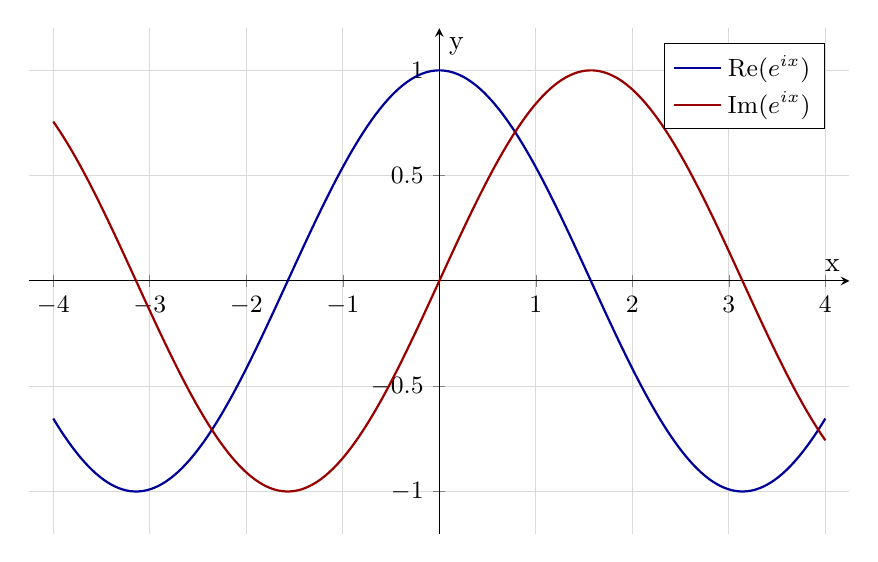
\begin{tikzpicture}
  \begin{axis}[
      xlabel={x},
      ylabel={y},
      xmin=-4.25, xmax=4.25,
      ymin=-1.2, ymax=1.2,
      grid=major,
      grid style={gray!30},
      axis lines=middle,
      width=12cm,
      height=8cm,
      xticklabel style={font=\small},
      yticklabel style={font=\small},
      legend pos=north east,
      legend style={font=\small}
    ]

    \addplot[
      domain=-4:4,
      samples=200,
      thick,
      blue!60!black
    ] {cos(deg(x))};
    \addlegendentry{$\operatorname{Re}(e^{ix})$}

    \addplot[
      domain=-4:4,
      samples=200,
      thick,
      red!60!black
    ] {sin(deg(x))};
    \addlegendentry{$\operatorname{Im}(e^{ix})$}

  \end{axis}
\end{tikzpicture}

      \vspace{0.5em}
      \captionof{figure}{Graph of $y = \exp(ix) = \cos(x) +
        i\sin(x)$, with the imaginary portion of $e^{ix}$ represented
      as $\operatorname{Im}(e^{ix})$.}
    }

\end{enumerate}

\pagebreak

\section*{Problem 2.6.3}

Consider the problem of an electron in a one-dimensional "infinite"
potential well of width $L_z$ in
the $z$ direction (i.e., the potential energy is infinite for $z < 0$ and
  for $z > L_z$, and, for simplicity, zero
for other values of $z$). For each of the following functions, in
exactly the form stated, is this function
a solution of the time-independent Schr\"odinger equation?

\begin{enumerate}[(i)]
  \item $\sin(7\pi z / L_z)$

    \boxedanswersmall{
      \centering
      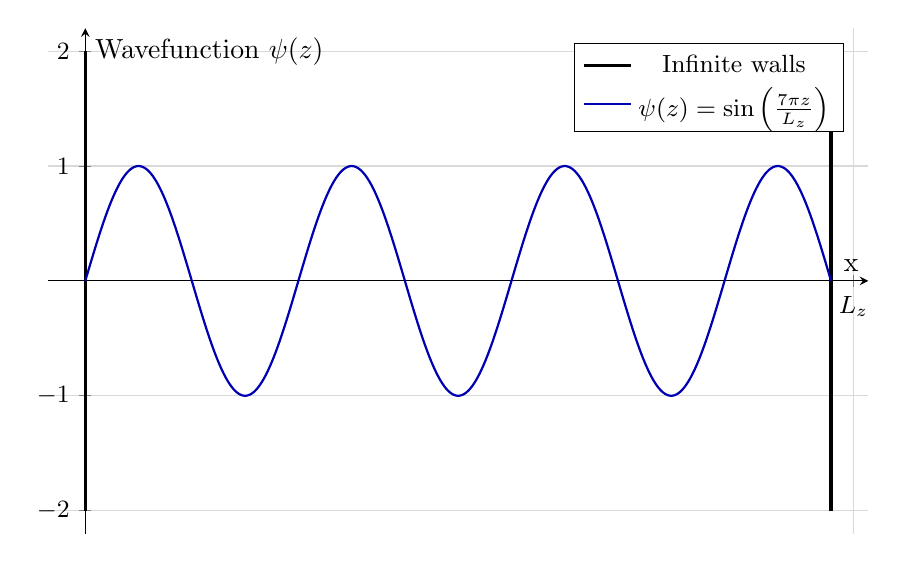
\begin{tikzpicture}
  \begin{axis}[
      xlabel={x},
      ylabel={Wavefunction $\psi(z)$},
      xmin=-0.05, xmax=1.05,
      ymin=-2.2, ymax=2.2,
      grid=major,
      grid style={gray!30},
      axis lines=middle,
      width=12cm,
      height=8cm,
      xtick={0, 1.03},
      xticklabels={0, $L_z$},
      xticklabel style={font=\small},
      yticklabel style={font=\small},
      legend pos=north east,
      legend style={font=\small}
    ]
    % Infinite potential walls (vertical lines)
    \addplot[black, very thick, domain=-0.2:2, samples=2] {-2.5}; %
    \addlegendentry{Infinite walls}
    \draw[black, very thick] (axis cs:0,-2) -- (axis cs:0,2);
    \draw[black, very thick] (axis cs:1,-2) -- (axis cs:1,2);

    % Wavefunction psi_7(z) = sin(7*pi*z/L_z)
    % For L_z = 1, this becomes sin(7*pi*z)
    \addplot[
      domain=0:1,
      samples=400,
      thick,
      blue!70!black
    ] {sin(deg(7*pi*x))};

    % Add legend entry
    \addlegendentry{$\psi(z) = \sin\left(\frac{7\pi z}{L_z}\right)$}

    % Add wall labels
    \node[black, above] at (axis cs:-0.1,1.8) {\small Wall};
    \node[black, above] at (axis cs:-0.1,1.8) {\small Wall};
  \end{axis}
\end{tikzpicture}

      \vspace{0.5em}
      \captionof{figure}{Graph of $\psi(z) = \sin\left(\frac{7\pi
      z}{L_z}\right)$}

      This fits the general (unnormalized) solution of the particle
      in an infinite well:

      \begin{equation*}
        \psi_n(z) = A_n\sin\left(\frac{n\pi
        z}{L_z}\right) \tag{2.25}
      \end{equation*}
    }

  \item $\cos(2\pi z / L_z)$

    \boxedanswersmall{
      \centering
      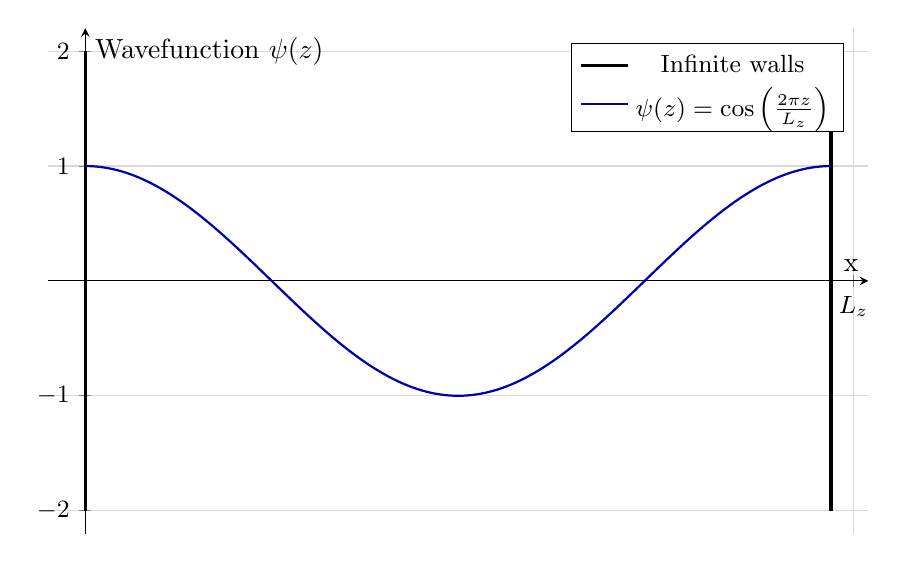
\begin{tikzpicture}
  \begin{axis}[
      xlabel={x},
      ylabel={Wavefunction $\psi(z)$},
      xmin=-0.05, xmax=1.05,
      ymin=-2.2, ymax=2.2,
      grid=major,
      grid style={gray!30},
      axis lines=middle,
      width=12cm,
      height=8cm,
      xtick={0, 1.03},
      xticklabels={0, $L_z$},
      xticklabel style={font=\small},
      yticklabel style={font=\small},
      legend pos=north east,
      legend style={font=\small}
    ]
    % Infinite potential walls (vertical lines)
    \addplot[black, very thick, domain=-0.2:2, samples=2] {-2.5}; %
    \addlegendentry{Infinite walls}
    \draw[black, very thick] (axis cs:0,-2) -- (axis cs:0,2);
    \draw[black, very thick] (axis cs:1,-2) -- (axis cs:1,2);

    % Wavefunction psi_7(z) = sin(7*pi*z/L_z)
    % For L_z = 1, this becomes sin(7*pi*z)
    \addplot[
      domain=0:1,
      samples=400,
      thick,
      blue!70!black
    ] {cos(deg(2*pi*x))};

    % Add legend entry
    \addlegendentry{$\psi(z) = \cos\left(\frac{2\pi z}{L_z}\right)$}

    % Add wall labels
    \node[black, above] at (axis cs:-0.1,1.8) {\small Wall};
    \node[black, above] at (axis cs:-0.1,1.8) {\small Wall};
  \end{axis}
\end{tikzpicture}

      \vspace{0.5em}
      \captionof{figure}{Graph of $\psi(z) = \cos\left(\frac{2\pi
      z}{L_z}\right)$.}

      This expression violates the the boundary conditions of the infinite well
      potential. Specifically, that the wavefunction should be zero
      at the walls.
      This expression has a value of 1 at both walls, therefore it is
      not a solution to the time-independent Schr\"odinger equation.
    }

\end{enumerate}

\pagebreak

\section*{Problem 2.7.1}

Which of the following pairs of functions are orthogonal on the
interval $-1$ to $+1$?

\begin{enumerate}
  \item[(i)] $x, x^2$

    \boxedanswersmall{

      Orthogonality is defined as follows:
      \begin{align*}
        \int_0^{L_z} g^*(z)h(z) dz = 0 \tag{2.32}
      \end{align*}

      Or on any other choice interval. In other words, if the inner
      product on a given interval is 0, then the two functions are
      orthogonal on that interval.

      \begin{align*}
        \int_{-1}^1 (x)(x^2) dx &= 0 \\
        \int_{-1}^1 x^3 dx &= 0 \\
        \left[\frac{x^4}{4}\right]_{-1}^1 &= 0 \\
        \left[(1)^4 - (-1)^4\right]_{-1}^1 &= 0 \\
        \Aboxed{0 &= 0}
      \end{align*}

      $x$ and $x^2$ are orthogonal on $[-1, 1]$

    }

  \item[(v)] $\exp(-2\pi ix), \exp(2\pi ix)$

    \boxedanswersmall{
      \begin{align*}
        \int_{-1}^1 (\exp(-2\pi ix))(\exp(2\pi ix)) dx &= 0 \\
        \int_{-1}^1 \exp(-2\pi ix + 2\pi ix) dx &= 0 \\
        \int_{-1}^1 \exp(0) dx &= 0 \\
        \int_{-1}^1 1 dx &= 0 \\
        \left[x\right]_{-1}^1 &= 0 \\
        \left[1 - (-1)\right] &= 0 \\
        \Aboxed{2 &\ne 0} \\
      \end{align*}
      $\exp(-2\pi ix)$ and $\exp(2\pi ix)$ are not orthogonal on $[-1, 1]$
    }

\end{enumerate}

\pagebreak

\section*{Problem 2.8.2}

An electron wave of energy \SI{0.5}{\electronvolt} is incident on an
infinitely thick potential barrier of height
\SI{1}{\electronvolt}. Is the electron more likely to be found (a) within the
first \SI{1}{\angstrom} of the barrier, or (b)
somewhere further into the barrier?

\boxedanswer{
  This can be determined by looking at the solution to this problem provided by:

  \begin{align*}
    \psi_{left}(z) &= C\exp(ikz) + D \exp(-ikz) \tag{2.40} \\
    k &= \sqrt{\frac{2mE}{\hbar^2}} \\
    D &= \frac{k - ik}{k + ik}C \tag{2.47} \\
    \psi_{right}(z) &= G \exp(-\kappa z) \tag{2.43} \\
    \kappa &= \sqrt{\frac{2m(V_0 - E)}{\hbar^2}} \\
    G &= \frac{2k}{k + i\kappa}C \tag{2.46} \\
  \end{align*}

  Because we are only considering relative probability, we do not need to
  normalize the wave function. So a value of $C = \SI{1}{\per\angstrom}$
  will be chosen
  for convenience. In addition, we only need to consider the
  right-hand side of the
  wave function.

  \begin{align*}
    % \psi_{left}(z) &= \exp\left(i\left[
    % \sqrt{\frac{2mE}{\hbar^2}}\right]z\right) + \exp\left(-ik\left[
    % \sqrt{\frac{2mE}{\hbar^2}}\right]z\right) \\
    \psi_{right}(z) &= \frac{2k}{k + i\kappa}\exp(-\kappa z) \tag{2.43} \\
    p_1 &= \int_0^l \psi_{right}(z) dz\\
    p_1 &= \int_0^l\left|\frac{2k}{k + i\kappa}\exp(-\kappa z)\right|^2dz\\
    p_1 &= \left|\frac{2k}{k +
    i\kappa}\right|^2\int_0^l\exp(-2\kappa z)dz\\
    p_1 &= \left|\frac{2k}{k +
    i\kappa}\right|^2\left[\frac{\exp(-2\kappa z)}{-2\kappa}\right]_0^l\\
    p_1 &= \left|\frac{2k}{k +
    i\kappa}\right|^2\left[\frac{\exp(-2\kappa l)}{-2\kappa} -
    \frac{1}{-2\kappa}\right]\\
    p_2 &= \left|\frac{2k}{k +
    i\kappa}\right|^2\left[-\frac{\exp(-2\kappa l)}{-2\kappa}\right]\\
    &
    \begin{aligned}
      k &= \sqrt{\frac{2mE}{\hbar^2}} \\
      \kappa &= \sqrt{\frac{2m(V_0 - E)}{\hbar^2}} \\
      m &= \SI{9.109e-31}{\kilo\gram} \\
      E &= \SI{0.5}{\electronvolt} = \SI{8.01e-23}{\joule} \\
      \hbar &= \SI{1.054e-34}{\joule\second} \\
      V_0 &= \SI{1}{\electronvolt} = \SI{1.602e-19}{\joule} \\
    \end{aligned} \\
  \end{align*}

}

\pagebreak

\boxedanswersmall{

  \begin{align*}
    \Aboxed{p_1 &= 1.4229} \\
    \Aboxed{p_2 &=  1.3376}
  \end{align*}

  It is more likely to find the electron within 1 Å of the wall,
as $1.4229 > 1.3376$.

  It is not significant that the "probabilities" are greater than one,
  as we did not
  normalize the wave function.
}

\section*{Supplemental Code}

Any computational aid was provided using a programming language
called \href{https://julialang.org}{Julia.} Source code is provided below.

\inputminted{julia}{./calculations/src/calculations.jl}

\end{document}
